\documentclass{beamer}
\usefonttheme{serif}
\usepackage{biblatex}
\usepackage{textcomp}
\usepackage{wrapfig}

\newcommand\blfootnote[1]{%
  \begingroup
  \renewcommand\thefootnote{}\footnote{#1}%
  \addtocounter{footnote}{-1}%
  \endgroup
}

\addtobeamertemplate{navigation symbols}{}{%
    \usebeamerfont{footline}%
    \usebeamercolor[fg]{footline}%
    \hspace{1em}%
    \insertframenumber/\inserttotalframenumber
}
\beamertemplatenavigationsymbolsempty
\setbeamercolor{footline}{fg=blue}
\setbeamerfont{footline}{series=\bfseries}
\setbeamertemplate{footline}[frame number]

\title{The Effect of Acquisition Resolution and \\ Magnetic Field Strength on \\ Multivariate Decoding \\ of fMRI}
\author{Ayan Sengupta}
\institute[Affiliations] % (optional)
{
  %
  Institute of Psychology\\
  Faculty of Natural Sciences\\
  Otto-von-Guericke University\\
  Magdeburg
}
%~ \titlegraphic{
\includegraphics[height=0.4cm]{Thesis_pictures/logo}\hfill}
\date{\today}




\begin{document}
\frame{\titlepage}


	%~ \begin{frame}
		%~ \frametitle{fMRI and Univariate Analysis}
		%~ \begin{center}
			%~ \includegraphics[height=5cm]{Thesis_pictures/general_introduction/GLM}
		%~ \end{center}
		%~ \begin{itemize}
			%~ \item Mass-univariate General Linear Model analysis
		%~ \end{itemize}
	%~ \end{frame}
    

	\begin{frame}
		\frametitle{Multivariate Decoding of fMRI}
		\begin{center}
			\includegraphics[height=6.5cm]{Thesis_pictures/general_introduction/MVPA}
		\end{center}
		\blfootnote{Reproduced from Haxby et al. 2014}
	\end{frame}
    

	\begin{frame}
		\frametitle{Multivariate Decoding of fMRI}
		\begin{center}
			\includegraphics[height=6.5cm]{Thesis_pictures/general_introduction/MVPA_2}
		\end{center}
		\blfootnote{Reproduced from Haxby et al. 2014}
	\end{frame}


	\begin{frame}
		\frametitle{What is a Classifier?}
		\begin{center}
			\includegraphics[height=5cm]{Thesis_pictures/classifier}
		\end{center}
		\begin{itemize}
			\item \textbf{Widely used Classifier: Linear Support Vector Machines}
		\end{itemize}
	\end{frame}


    
	\begin{frame}
		\frametitle{Decoding Orientation from primary visual cortex (V1): Extensively used decoding paradigm}
		\begin{center}
			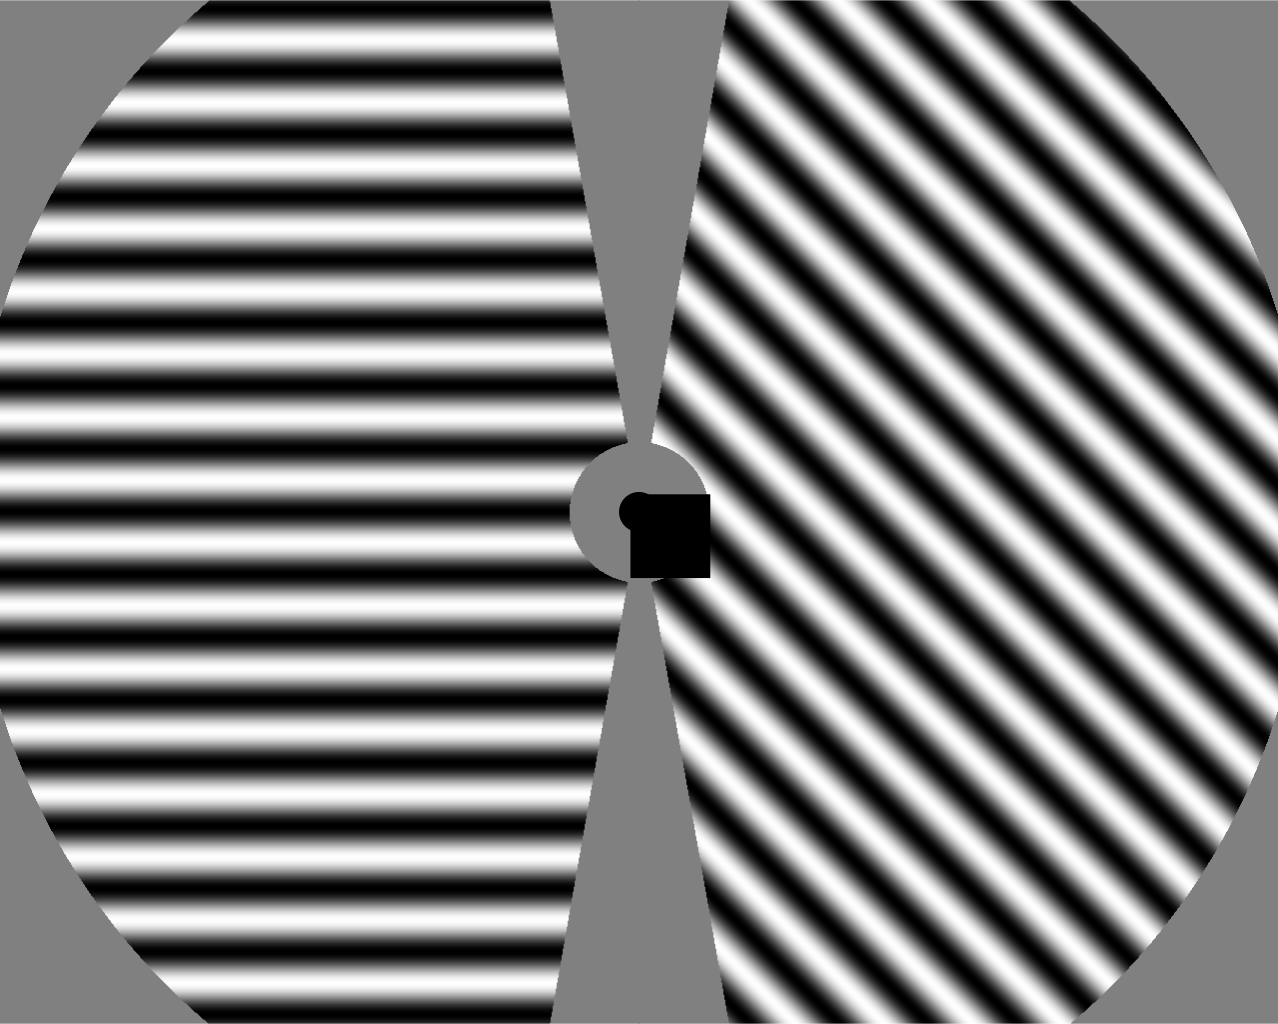
\includegraphics[height=3cm]{Thesis_pictures/exp_frame}
		\end{center}
		\begin{itemize}
			\item Initial studies: Kamitani and Tong (2005), Haynes and Rees (2005)
			\item Chaimow et al.(2010), Swisher et al.(2010), Alink et al.(2013), 
			Freeman et al.(2013) studied spatial scale of orientation decoding signals
			\item Acquisition resolution of 3mm iso.
		\end{itemize}
	\end{frame}
  
  
	\begin{frame}
		\frametitle{Spatial Scale of Orientation decoding Signals: Why is it relevant?}
		\begin{center}
			\includegraphics[height=3cm]{Thesis_pictures/partial_volume}
		\end{center}
		\begin{itemize}
			\item Presence of sub-millimeter structures called orientation 
			columns (Hubel and Wiesel (1972), Braitenberg and Braitenberg (1979)).
			\item Partial volume effect (Weibull et al., 2008) leads to 
			averaging of signals from multiple orientation columns into a standard 3mm iso voxel.
		\end{itemize}
	\end{frame}
	
	
	
	%~ \begin{frame}
	%~ \frametitle{Spatial Scale of Orientation Specific Signals}
		%~ \begin{itemize}
		 %~ \item \textbf{Aliasing of High Spatial Frequency Components} by inadequate
		 %~ sampling of larger voxels (Boynton et al., 2005, Alink et al., 2013).
		 %~ \item \textbf{"Biased Draining Regions" of macroscopic veins} \\(Gardner et al., 2006, Shmuel et al., 2010).
		 %~ \item \textbf{Random, local variations and irregularities} 
		 %~ in the functional organization \\(Kamitani and Tong, 2005, 2006, 
		 %~ Haynes and Rees, 2006, Kriegeskorte and Bandettini, 2007)
		%~ \end{itemize}  
	%~ \end{frame}


	\begin{frame}
		\frametitle{Motivations behind multi-resolution UHF (7T) fMRI for Orientation Decoding}
		\begin{itemize}
		
			\item Higher the resolution $->$ Better sampling of the underlying neural signals \\
					Better signal $->$ Improved Decoding Accuracy
					
			\item  7T fMRI acquisition provides improved BOLD SNR for 
			resolutions $<$ 1mm iso leading to decreased partial volume effect.
			
			\item Yacoub et al. (2008) used high field (7T) fMRI to model pinwheel structures of 
			orientation columns in humans: But no orientation decoding
			
			\item The effect of acquisition resolution on multivariate decoding 
			performance is an unexplored territory.
			
			%~ \item Conclusion about the spatial scale of the orientation 
			%~ specific signals in previous studies were performed by fMRI acquisition in one particular 
			%~ resolution followed by Volumetric Gaussian filtering with different kernel 
			%~ width (expressed in FWHM).

			 %~ Studying this is extremely relevant keeping in mind the 
			 %~ widely debated topic of the true spatial frequency, 
			 %~ because sampling of the underlying neural signals directly 
			 %~ affected by the acquisition resolution  
		\end{itemize}
	\end{frame}	


	\begin{frame}
		\begin{center}
			\Large Experiment 1: The Effect of Acquisition Resolution on Orientation Decoding
		\end{center}
	\end{frame}

    \begin{frame}
        \frametitle{Stimulus}
            \begin{center}
                \includegraphics[height=4cm]{Thesis_pictures/experiment_1/figure_1}
            \end{center}
            \begin{itemize}
                \item 30 Trials = 1 Experimental run
                \item Number of runs = 10
                \item Total scan time = 40min
                \item 4 orientations in each hemifield (0\textdegree, 45\textdegree, 90\textdegree \& 135\textdegree) with random phase shifts
            \end{itemize}
    \end{frame}




	\begin{frame}
		\frametitle{Acquisition Protocols}
		\begin{center}
			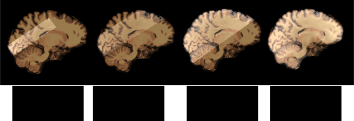
\includegraphics[height=3cm]{Thesis_pictures/acquisition}
		\end{center}
		\begin{itemize}
		 \item Number of participant: 7		
		 \item Siemens 7 Tesla scanner with 32 channel head coil (Nova Medical, Wilmington, MA)
		 \item T2*-weighted echo planar images (EPI) (TR/TE=2000/22 ms, FA=90\textdegree)
		 \item Sequential acquisitions with 10\% inter-slice gap parallel to calcarine sulcus (on a tilted 
		 axial plane)
		\end{itemize}  
	\end{frame} 

  
 
    
  \begin{frame}
    \frametitle{Region of interest localization}
        \begin{center}
            \includegraphics[height=4.5cm]{Thesis_pictures/ROI_retmap}
        \end{center}
        \begin{itemize}
			\item Retinotopic mapping to delineate V1 region. \\(data acquired from \textit{studyforrest.org})
        \end{itemize} 
        \blfootnote{published in Sengupta et. al. 2016 \textit{Nature Scientific Data}}
    \end{frame} 
    
  \begin{frame}
    \frametitle{Classification Results (V1)}
        \begin{center}
            \includegraphics[height=5cm]{Thesis_pictures/classification_result}
        \end{center}
        \begin{itemize}
			\item \textbf{Non-Linear relation between Acquisition Resolution and Decoding Accuracy}
        \end{itemize} 
        \blfootnote{Sengupta et al. \textit{Neuroimage} (under review)}
    \end{frame}

  %~ \begin{frame}
    %~ \frametitle{Classification Results (Fixed Number of Voxels)}
        %~ \begin{center}
            %~ \includegraphics[height=4.5cm]{Thesis_pictures/fixed_voxel}
        %~ \end{center}
    %~ \end{frame}    

   

  %~ \begin{frame}
    %~ \frametitle{Mean Pecrentage BOLD signal change}
        %~ \begin{center}
            %~ 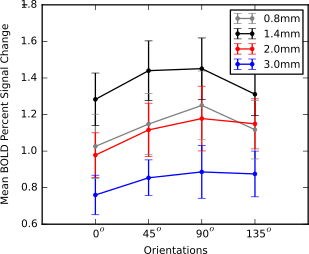
\includegraphics[height=6cm]{../pictures/signal_change}
        %~ \end{center}
    %~ \end{frame} 


  \begin{frame}
    \frametitle{Spatial Filtering Steps}
        \begin{center}
            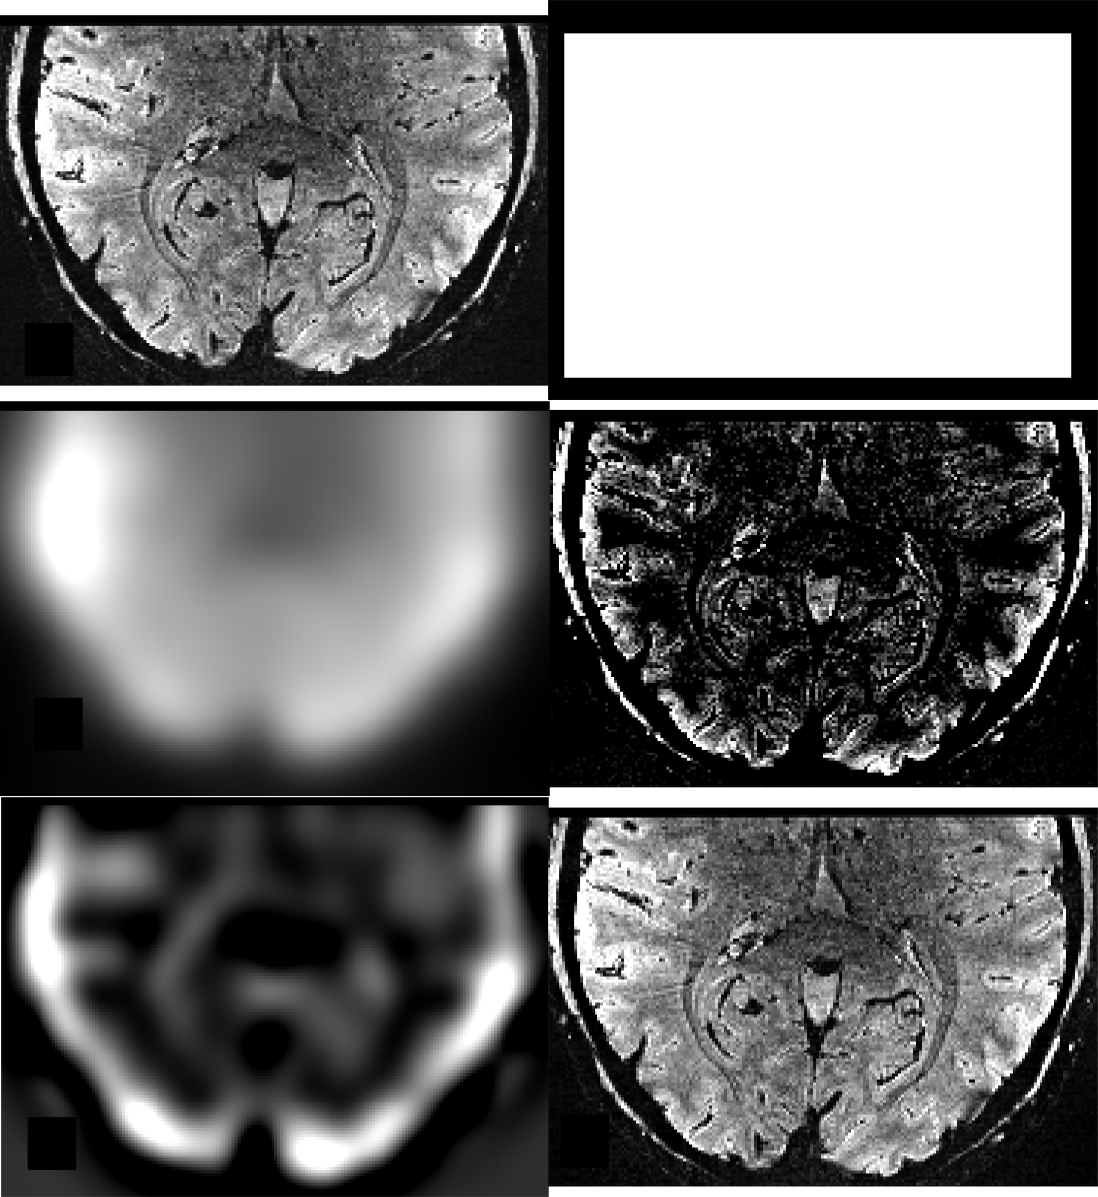
\includegraphics[height=5cm]{Thesis_pictures/filtering_steps}
        \end{center}
        \blfootnote{Sengupta et al. \textit{Neuroimage} (under review)}
    \end{frame} 

  \begin{frame}
    \frametitle{Classification Results after Spatial Filtering}
        \begin{center}
            \includegraphics[height=5.5cm]{Thesis_pictures/LPF}
        \end{center}
        \blfootnote{Sengupta et al. \textit{Neuroimage} (under review)}
    \end{frame} 

  \begin{frame}
    \frametitle{Classification Results after Spatial Filtering}
        \begin{center}
            \includegraphics[height=5.5cm]{Thesis_pictures/HPF}
        \end{center}
        \blfootnote{Sengupta et al. \textit{Neuroimage} (under review)}
    \end{frame} 

  \begin{frame}
    \frametitle{Classification Results after Spatial Filtering}
        \begin{center}
            \includegraphics[height=5.5cm]{Thesis_pictures/BPF}
        \end{center}
        \blfootnote{Sengupta et al. \textit{Neuroimage} (under review)}
    \end{frame} 


  \begin{frame}
    \frametitle{Classification Results after Spatial Filtering}
        \begin{center}
            \includegraphics[height=5.5cm]{Thesis_pictures/spatial_smoothing_multires}
        \end{center}
        \begin{itemize}
			\item \textbf{Broadband nature} of Orientation specific signals
			 \item No evidence of \textbf{Aliasing of High Spatial Frequency Components} by inadequate
			 sampling of larger voxels (Boynton et al., 2005, Alink et al., 2013).
        \end{itemize}
    \end{frame} 

  %~ \begin{frame}
    %~ \frametitle{Spatial Re-sampling to Other Resolutions}
        %~ \begin{center}
            %~ 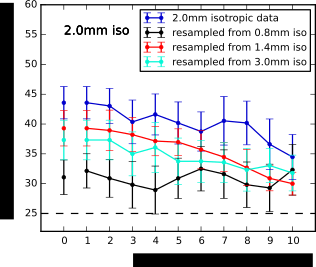
\includegraphics[height=7cm]{../pictures/resampling}
        %~ \end{center}
    %~ \end{frame}

  \begin{frame}
    \frametitle{Contribution of veins to decoding}
        \begin{center}
            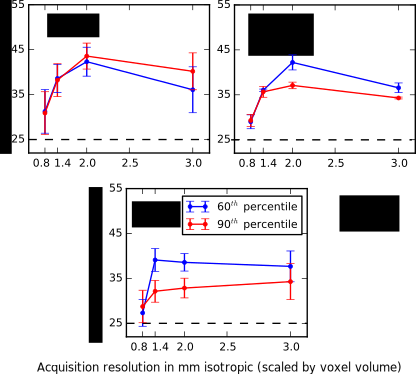
\includegraphics[height=3.5cm]{Thesis_pictures/veins}
        \end{center}
        \begin{itemize}
			\item \textbf{Susceptibility Weighted Imaging} data to localize veins \\(data acquired from \textit{studyforrest.org})
			\item \textbf{Biased Draining Regions} of macroscopic veins 
			contribute to orientation decoding (Gardner et al., 2006, Shmuel et al., 2010).
		\end{itemize}
    \end{frame} 

  \begin{frame}
    \frametitle{Dependence on temporal Signal to Noise Ratio (tSNR)}
        \begin{center}
            \includegraphics[height=5cm]{Thesis_pictures/tSNR}
        \end{center}
        \begin{itemize}
			\item \textbf{Balance of tSNR and sampling frequency of 
			Acquisition Resolution drive Orientation decoding accuracy}
		\end{itemize}

    \end{frame} 
    
    
  %~ \begin{frame}
    %~ \frametitle{Recap: Effect of Acquisition Resolution}
        %~ \begin{center}
            %~ \includegraphics[height=7cm]{Thesis_pictures/classification_result}
        %~ \end{center}
    %~ \end{frame}



	\begin{frame}
		\frametitle{Motivations behind comparison of 7T and 3T fMRI for Orientation Decoding}
		\begin{itemize}
			\item The best performing 2mm iso resolution can be acquired 
			with good SNR in 3T.
			\item Effect of Magnetic field strength on orientation decoding 
			has not been explored yet.
		\end{itemize}
	\end{frame}	


	\begin{frame}
		\begin{center}
			\Large Experiment 2: The Effect of Magnetic Field Strength on Orientation Decoding
		\end{center}
	\end{frame}




	\begin{frame}
		\frametitle{Acquisition Protocols}
		\begin{itemize}
		 \item Siemens 3 Tesla Prisma scanner with 64 channel head coil (Siemens, Erlangen, Germany)
		 \item Acquisition resolutions: 1.4mm iso, 2.0mm iso and 3.0mm iso
		 \item T2*-weighted echo planar images (EPI) (TR/TE=2000/30 ms, FA=90\textdegree)
		 \item \textbf{Protocols unaltered} with minimum modifications
		 \item Number of subjects: 7 (\textbf{5 out of 7} subjects participated in both experiments)
		\end{itemize}  
	\end{frame} 


  \begin{frame}
    \frametitle{Decoding Analysis Procedure}
		\begin{itemize}
		 \item \textbf{Feature selection} : Univariate analysis done to determine 
		 the visually responsive voxels in V1 and decoding was performed on it.
		 \item \textbf{Consistency:} 7T data acquired in 1.4mm iso, 2.0mm iso and 3.0mm iso \textbf{re-analyzed} 
		 with the same processing pipeline.
		\end{itemize}  
    \end{frame}


  \begin{frame}
    \frametitle{Orientation Decoding Performance 7T vs 3T}
        \begin{center}
            \includegraphics[height=5cm]{Thesis_pictures/7T_3T_comparisons}
        \end{center}
		\begin{itemize}
		 \item 7T results are \textbf{similar}.
		 \item Decoding accuracy in 3T data shows \textbf{linear dependence} on acquisition resolution.
		 \item \textbf{3mm iso data} show \textbf{identical performance} across Field strength.
		\end{itemize} 
    \end{frame}


  \begin{frame}
    \frametitle{Comparison of tSNR 7T vs 3T}
        \begin{center}
            \includegraphics[height=5cm]{Thesis_pictures/7T_3T_tSNR}
        \end{center}
        \begin{itemize}
			\item Mean tSNR values and fitted model \textbf{similar} as in Triantafyllou et al.{2011}.
			\item Differences in decoding performance across field strength is a reflection of tSNR differences.
		\end{itemize}
    \end{frame}


  \begin{frame}
    \frametitle{Does improvement of tSNR on 3T acquisition makes decoding performance comparable to 7T ?}
        \begin{center}
            \includegraphics[height=5cm]{Thesis_pictures/experiment_3/figure_1}
        \end{center}
        \begin{itemize}
			 \item Removal of parallel imaging (SENSE 2)
			 \item Introduction of multislice parallel acquisition (MB factor 2)
			 \item 38.45\% increase in tSNR but 3\% of increase in decoding accuracy
		\end{itemize}  
    \end{frame}


  \begin{frame}
    \frametitle{Generality of the findings across different ROIs in the brain}
        
        \begin{center}
            \includegraphics[height=5cm]{Thesis_pictures/appendix_1/figure_1}
        \end{center}
        \begin{itemize}
			 \item Decoding of musical genres in human primary auditory cortex
			 \item Spatial smoothing reveals similar patterns in the suditory cortex 
			 as in the visual cortex.
		\end{itemize}  
    \end{frame}



  \begin{frame}
    \frametitle{Conclusions}
        %~ \begin{center}
        %~ \begin{itemize}
         %~ \item Optimal Acquisition Resolution is $\approx$ 2.5mm iso.
         %~ \item Aliasing is improbable. Highest accuracy of band-pass 
         %~ components $\approx$ 5-8mm FWHM for all resolutions.
         %~ \item Low spatial frequency components contribute to noise.
         %~ \item Down-sampling high resolution fMRI into lower resolutions 
         %~ does not help decoding, orientation signal not exclusively high frequency.
         %~ \item Veins carry little orientation specific signal.
        %~ \end{itemize}  
        %~ \end{center}
    \end{frame} 


  \begin{frame}
    \frametitle{Future Research}

    \end{frame}




  %~ \begin{frame}
    %~ \frametitle{Acknowledgements}
        %~ \begin{itemize}
         %~ \item Jun. Prof. Dr. Michael Hanke
         %~ \item Renat Yakupov
         %~ \item Prof. Dr. Stefan Pollmann
         %~ \item Prof. Dr. Oliver Speck
        %~ \end{itemize}
        %~ \vspace{1cm}
        %~ \begin{center} 
            %~ 
\includegraphics[height=1.5cm]{../pictures/funding}
        %~ \end{center}
    %~ \end{frame}


  %~ \begin{frame}
        %~ \begin{center}
            %~ Questions
        %~ \end{center}
    %~ \end{frame} 
    
  %~ \begin{frame}
    %~ \frametitle{Discussion: Nyquist Sampling Theory}
        %~ \begin{center}
            %~ 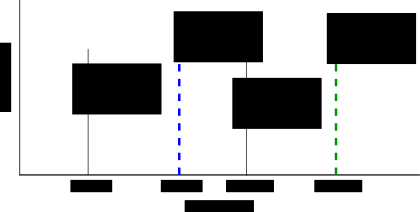
\includegraphics[height=5cm]{../pictures/nyquist}
        %~ \end{center}
    %~ \end{frame}                 
    
    
     
  %~ \begin{frame}
    %~ \frametitle{General Workflow of Orientation decoding analysis}
        %~ \begin{itemize}
            %~ \item EPI acquisition in one particular resolution
            %~ \item Volumetric Gaussian filtering with increase in kernel width (expressed in FWHM)
            %~ \item Within-subject leave-one-run-out cross-validation with LinearSVM classifier
            %~ \item Conclusion about the spatial scale of the Orientation specific signals 
        %~ \end{itemize}  
    %~ \end{frame}

  %~ \begin{frame}
    %~ \frametitle{High field fMRI unveils orientation columns in humans}
        %~ \begin{center}
            %~ 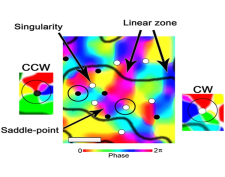
\includegraphics[height=4cm]{../pictures/Yacoub_pinwheel}
        %~ \end{center}
        %~ \begin{itemize}
            %~ \item Yacoub et al. (2008) used high field strength (7T)
            %~ \item Voxel dimensions - 0.5mm x 0.5mm x 3.0mm
            %~ \item The pinwheel pattern maps were reproducible
        %~ \end{itemize}  
    %~ \end{frame}

  %~ \begin{frame}
    %~ \frametitle{Impressions about Optimal Acquisition Resolution}
        %~ \begin{itemize}
            %~ \item Smaller the voxel size = Better Orientation Signals from the Orientation Columns
            %~ \item If sub-millimeter columnar structures are exclusive sources of classification information 
            %~ then decoding will not be possible when voxel size is 3mm iso or when volumetric spatial 
            %~ smoothing is performed.
        %~ \end{itemize}  
    %~ \end{frame}


  %~ \begin{frame}
    %~ \frametitle{Spatial smoothing does not hurt Orientation decoding}
        %~ \begin{center}
            %~ 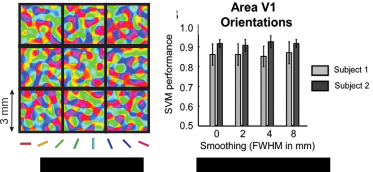
\includegraphics[height=4cm]{../pictures/grid_3mm_op_de_beeck}
        %~ \end{center}
        %~ \begin{itemize}
            %~ \item Reliable Orientation decoding is possible with 3mm iso voxel size. (Kamitani and Tong, 2005 and Haynes and Rees, 2005)
            %~ \item Above chance level decoding could be performed after spatial Gaussian smoothing.
        %~ \end{itemize}  
    %~ \end{frame}

  %~ \begin{frame}
    %~ \frametitle{Spatial scale of Orientation specific signals}
        %~ \begin{center}
            %~ \includegraphics[height=4cm]{../pictures/swisher}
        %~ \end{center}
        %~ \begin{itemize}
         %~ \item fMRI activity patterns can be found at spatial scales 
         %~ from the size of individual columns to about a centimeter 
         %~ (Swisher et al., 2010).
        %~ \end{itemize}  
    %~ \end{frame}



  %~ \begin{frame}
    %~ \frametitle{Simulation Study by Chaimow et al., 2010}
        %~ \begin{center}
            %~ 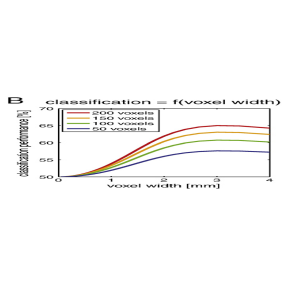
\includegraphics[height=5.5cm]{../pictures/shmuel_model}
        %~ \end{center}
        %~ \begin{itemize}
         %~ \item Chaimow et al., 2010 simulated fMRI data to model decoding 
         %~ of ODCs at different acquisition resolutions.
        %~ \end{itemize}  
    %~ \end{frame}
       
\end{document}
